\documentclass{article}

% Language setting
% Replace `english' with e.g. `spanish' to change the document language
\usepackage[english]{babel}

% Set page size and margins
% Replace `letterpaper' with `a4paper' for UK/EU standard size
\usepackage[letterpaper,top=2cm,bottom=2cm,left=2.5cm,right=3cm,marginparwidth=1.75cm]{geometry}

% charts
\usepackage{tikz}
\usepackage{pgfplots}
\pgfplotsset{compat=1.17}
\usetikzlibrary{intersections} 

% Useful packages
\usepackage{amsmath}
\usepackage{graphicx}
\usepackage[table]{xcolor}
\usepackage[colorlinks=true, allcolors=blue]
{hyperref}


\usepackage[
backend=biber,
style=ieee,
]{biblatex}

\title{Case Study: Innovating in the Connected Mobility Industry.
}
\author{Aleksandr Petrunin}

\addbibresource{sample.bib} %Imports bibliography file

\begin{document}

% ---------------------------
% Title page (custom)
% ---------------------------
\begin{titlepage}
  \begin{center}
    \includegraphics[width=5cm]{nup_logo.png} \\[1cm]
    {\Large Neapolis University Pafos} \\[0.5cm]

    {\large \textbf{Course Code:} IS507} \\[2cm]

    {\huge \textbf{Case Study: Innovating in the Connected Mobility Industry.}} \\[1.5cm]

    {\large \textbf{Name:} Aleksandr Petrunin} \\[0.3cm]
    {\large \textbf{Student ID:} 1251114137} \\[2cm]

    {\large \today}
  \end{center}
\end{titlepage}

\newpage
\tableofcontents

\newpage
\section{Introduction}
\textbf{UrbanMove} is a fast-growing European company offering electric scooters, shared e-bikes, and micro-mobility data services to municipalities. Founded in 2017, the company quickly expanded across major European cities by providing convenient, app-based transportation with real-time location and usage tracking.
\\\\
However, by 2025 UrbanMove is facing significant challenges:

\begin{itemize}
    \item Intense competition from global mobility giants using more advanced AI and predictive analytics.

    \item Regulatory pressure from cities demanding improved safety, sustainability, and data transparency.

    \item Rising operational costs due to device maintenance, vandalism, and fleet redistribution.

    \item Consumer expectations for connected, personalised, and seamless mobility experiences.
\end{itemize}

To remain competitive, UrbanMove's leadership has launched \textbf{Project Nexus}, a three-year strategic innovation initiative aiming to transform the company into a leader in connected mobility systems. Project Nexus contains four streams:

\begin{enumerate}
    \item Emerging Technology Intelligence

    \begin{itemize}
        \item Developing capabilities to identify, analyse, and adopt new disruptive technologies.
    \end{itemize}

    \item AI-Driven Operations
    \begin{itemize}
        \item Implementing machine learning and predictive maintenance models to reduce fleet downtime.
    \end{itemize}

    \item IoT-Enhanced Fleet Ecosystem
    \begin{itemize}
        \item Upgrading every scooter and bike with next-generation sensors, telematics, and edge-processing capabilities.
    \end{itemize}

    \item Crowdsourced Innovation \& Funding
    \begin{itemize}
         \item Engaging users and communities in co-creating new features, and exploring crowdfunding options for green infrastructure expansion.
    \end{itemize}
\end{enumerate}

As the Digital Transformation Officer, you have been asked to evaluate Project Nexus and provide an integrated analysis to support strategic decision-making.


\newpage
\section{Project evaluation and integrated analysis}
\subsection{Technological Innovation and Disruption}

\subsubsection{Connected mobility industry evolution}
\begin{itemize}
    \item Connected mobility industry is evolving toward integrating various transport means into one comprehensive system, replacing separate information, booking, and ticketing systems for competing modes. \cite{bongaerts2016disruption}
    \item Theoretical Framework for Disruption: Uses the Technology Acceptance Model (TAM) and value theory to provide a theoretical framework for understanding the adoption of disruptive innovations, including those in the mobility sector.
    \cite{bongaerts2016disruption}
    \item Blockchain and Connected Mobility: Identifies the development of blockchain technology as a potential new impulse for connected mobility, possibly rendering traditional intermediary business models obsolete through smart contracts.
    \cite{bongaerts2016disruption}
    \item Ideal Types of Mobility Services: Identifies three ideal types of innovative mobility services: 'mobility service added to product,' 'robotaxi,' and 'territorialized open mobility platform,' where the latter two have the potential to destabilize the automotive industry's architecture.
    \cite{alochet2020technological}

    \textbf{However}
        \item The transition to Battery Electric Vehicles (BEVs) is not making the industry as modular as predicted, which is reflected in the organizational structure of assembly and industry architecture, despite efforts by new entrants to modularize.
    \cite{jacobides2023revisiting}
    \item Jacobides et al. \cite{jacobides2023revisiting} propose a new theoretical structure for innovation, called "Mark III," which characterizes the connected mobility sector as one where incumbents and new entrants have a much tighter connection, involving acquisitions, alliances, and ecosystem formation.
    \cite{jacobides2023revisiting}
\end{itemize}


\raggedright
\subsubsection{What characteristics of UrbanMove`s environment make it particularly vulnerable to disruption?}
\begin{itemize}
\item Electrification and Industry Disruption: Confirms that vehicle electrification, a systemic innovation, is not enough alone to destabilize the industry, but its massification combined with other factors could lead to a disruptive dynamic, aligning with sociotechnical transition theory.
\cite{alochet2020technological}
\item Challenges in Car IT Transformation: Identifies the difficult and slow transformation of car IT as a specific area where the industry struggles, intensifying the speed of disruption and making established companies vulnerable.
\cite{winkelhake2018digital}
\item New Digital Competitors: Attributes the growing momentum of disruption to new market competitors, such as Tesla and other companies entering from the IT sector, that are 'born on the web' and lack the legacy structures of established manufacturers.
\cite{winkelhake2018digital}
\item Organizational Transformation Needs: Identifies that the need for organizational transformation and continuous education is often undervalued by the industry when productizing new emerging technologies, making them vulnerable to failure and collapse.
\cite{hamid2022autonomous}
\item Changing Ownership Models: Notes that the industry is rapidly deploying new forms of carsharing, ridesharing, and ridehailing services, which will reduce the importance of private vehicle ownership, indicating a vulnerability due to changing consumption models.
\cite{hamid2022autonomous}
\item Uncertainty in Trends: Identifies great uncertainty regarding technological evolution and social trends that will condition businesses in the near future as a major vulnerability.
\cite{turienzo2023business}
\item CAV Disruptive Potential: Notes that the disruptive potential of Connected and Autonomous Vehicles (CAV) has the capacity to transform existing business models, making them vulnerable.
\cite{turienzo2023business}
\end{itemize}

\raggedright
\subsubsection{To what extent could Project Nexus help UrbanMove avoid being displaced by competitors?}

\rowcolors{3}{gray!10}{gray!20}
\begin{tabular}{ |p{2cm}|p{4cm}|p{5cm}|p{4cm}|p{1.2cm}  |}

 \hline
 \multicolumn{5}{|c|}{Feasibility of Project Nexus: Problem-Solution Fit} \\
 \hline
 Challenge & Current Impact & How Project Nexus solves it & Evidence/Assumptions & Coverage \\
 \hline

 Competition & More advanced AI and predictive analytics & Stream 1 - to keep innovation, 2 - advancing AI, 3 - more data for analytics, 4 - faster feedback loop & All 4 streams complement mitigation of the competition challenge.& 100\%\\

 Regulations & Demanding improved safety, sustainability, and data trans-
parency & Stream 1, 3 - data for transparency & Safety and sustainability concerns are not addressed.& 33\% \\

 Operational costs & Rising due to device maintenance, vandalism, and fleet redistribution & Stream 1, 2 - mitigating maintenance, & Vandalism issue is not addressed. Fleet redistribution depends on the supply chain, not only fleet downtime.& 50\%\\
 
 Consumer expectations & Want connected, personalised, and seamless mobility experiences & Stream 1, 4 - feature co-creation & Connected and seamless terms are too abstract, probably SMART re-evaluation is needed.& 33\% \\
 
 \hline
\end{tabular}


\paragraph{Summary}
Project Nexus effectively addresses UrbanMove's challenges related to competition. However, a more detailed proposition and mitigation alignment would be beneficial for a 3-year project.

Despite securing the competitor displacement issue, other challenges are poorly covered and do not present an actionable resolution.

\newpage
\subsection{Sources of Innovation and Technological Development}

\subsubsection{Evaluation of UrbanMove’s internal and external sources of innovation.}

\paragraph{Internal sources of innovation}
\begin{enumerate}
    \item Operational Data Assets: UrbanMove possesses valuable real-time location and usage tracking data from its existing fleet operations, providing insights into user behavior, demand patterns, and operational inefficiencies.
    \item Fleet Management Expertise: Years of experience managing scooters and e-bikes across multiple European cities has developed organizational knowledge in logistics, redistribution, and urban mobility operations.
    \item Legacy Technology Debt: Current fleet lacks advanced sensors and analytics capabilities, suggesting historical underinvestment in R\&D and technological infrastructure.
    \item Limited AI/ML Capabilities: The competitive disadvantage against "global mobility giants using more advanced AI" indicates insufficient internal data science and machine learning expertise.
    \item Reactive Rather Than Proactive: The company appears to be responding to competitive and regulatory pressures rather than driving innovation from within, suggesting weak internal innovation culture.
\end{enumerate}

\paragraph{External sources of innovation}
\begin{enumerate}
    \item Technology Partnerships: Opportunities to collaborate with IoT sensor manufacturers, edge computing providers, and AI/ML platform vendors to rapidly upgrade technical capabilities.
    \item University and Research Collaborations: Access to European research institutions specializing in smart cities, mobility systems, and sustainable transportation for applied research partnerships.
    \item Open Innovation Platforms: The planned "Crowdsourced Innovation \& Funding" stream represents a structured approach to tap user creativity and community knowledge.
    \item Supplier Innovation: Next-generation telematics and sensor providers can contribute technological advancements developed for adjacent industries (automotive, logistics, smart cities).
    \item Regulatory Bodies as Innovation Drivers: City requirements for safety, sustainability, and data transparency can serve as forcing functions that drive innovation priorities.
    \item Industry Consortia and Standards Bodies: Participation in mobility-as-a-service (MaaS) platforms and interoperability initiatives provides access to shared innovation and best practices.
    \item Monitoring and learning from global mobility giants' technological deployments provides a roadmap for relevant innovations without full R\&D investment.
\end{enumerate}


\newpage
\subsubsection{Which sources of innovation are most relevant for UrbanMove?}
\paragraph{External Technology Partnerships (Highest Priority)} UrbanMove faces an urgent need to close the technology gap with competitors. Building advanced AI/ML capabilities and next-generation IoT infrastructure internally would require years and substantial investment the company may not afford given competitive pressures.

\paragraph{Crowdsourced and User-Driven Innovation (Strategic Differentiator)} This aligns directly with Stream 4 and represents a potential competitive advantage. As the proposal notes, the connected mobility industry is shifting toward user expectations for "connected, personalised, and seamless mobility experiences." User communities can identify pain points and desired features that purely technology-driven approaches might miss. While competitors may have superior technology, UrbanMove can differentiate through community engagement and co-creation, building user loyalty while generating innovation insights.

\paragraph{Operational Data as Internal Innovation Engine (Underutilized Asset)} UrbanMove's existing operational data represents an underexploited internal source. With proper analytics infrastructure (likely through external partnerships), this data can drive:
\begin{itemize}
    \item Predictive maintenance models
    \item Demand forecasting and dynamic redistribution
    \item Usage pattern analysis for service optimization
    \item Safety and risk assessment
\end{itemize}

\paragraph{Regulatory Requirements as Innovation Catalyst (Often Overlooked)} Rather than viewing regulatory pressure as purely a constraint, UrbanMove should engage proactively with municipalities to co-develop solutions. Cities seeking "improved safety, sustainability, and data transparency" can become innovation partners, providing clear requirements and potentially pilot funding.

\subsubsection{How could the company strengthen its innovation capabilities to accelerate Project Nexus?}
\paragraph{Establish a Dedicated Innovation Lab:} Create a cross-functional team focused on rapid prototyping and experimentation with emerging technologies relevant to connected mobility. Identify and collaborate with leading AI/ML firms, IoT sensor manufacturers, and edge computing providers to access cutting-edge capabilities without full internal development.
\paragraph{Invest in Data Analytics Infrastructure:} Build robust data pipelines and analytics platforms to fully leverage operational
data for predictive insights and optimization.
\paragraph{Cultivate an Open Innovation Culture:} Encourage stakeholders at all levels to contribute ideas and participate
in co-innovation initiatives, joint pilor programs, shared funding.
\begin{itemize}
    \item Engage with Regulatory Bodies: Proactively collaborate with city governments to align innovation efforts with regulatory
requirements and explore pilot opportunities.
    \item Leverage User Communities: Implement structured mechanisms for gathering user feedback and co-creating new features through crowdsourcing platforms.
\end{itemize}

\paragraph{Continuous Learning and Development:} Invest in upskilling internal teams on emerging technologies and innovation methodologies to build internal capabilities over time.
    


\newpage
\subsection{Technology Evaluation and Life Cycle Positioning}
\subsubsection{TLC and S-curve positioning}
Current E-technologies are approaching the plateau of the S-curve where further investment yields minimal competitive advantage.
\\Current telematics are maturing, but next-generation IoT (Stream 3) represents a new technology cycle entering early growth phase.
\\ AI implies high ROI potential; technology still in the phase where investment yields substantial performance gains.
\\ Innovations such as blockchain, Edge AI, autonomous systems are high risk but potential for first-mover advantage and industry reshaping.



\begin{center}
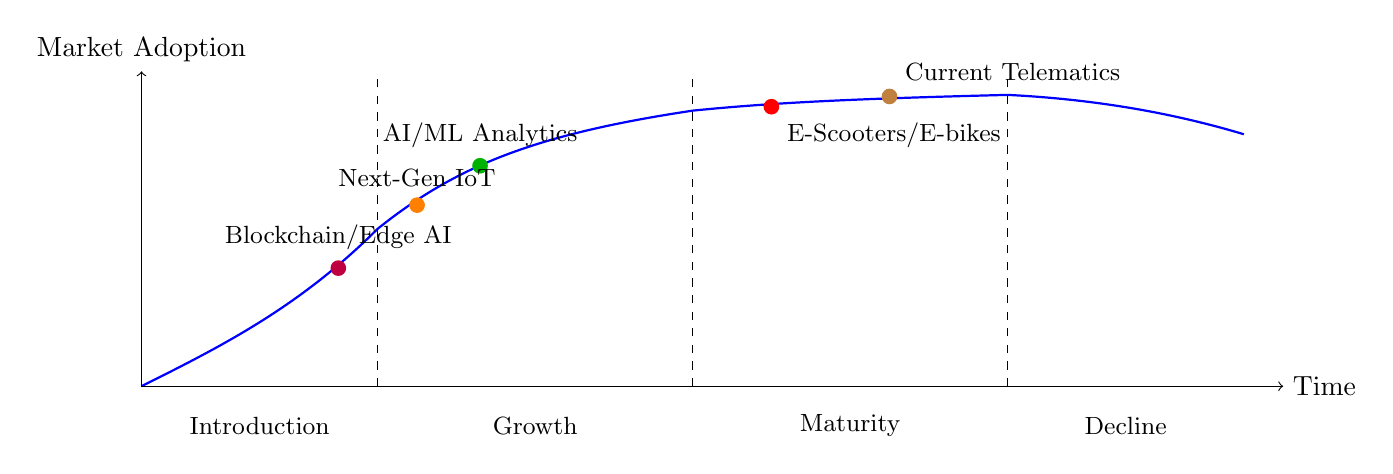
\begin{tikzpicture}[scale=1]
    % Draw the main curve
    \draw[thick, blue] (0,0) 
        .. controls (1,0.5) and (2,1) .. (3,2)
        .. controls (4,2.8) and (5,3.2) .. (7,3.5)
        .. controls (8,3.6) and (9,3.65) .. (11,3.7)
        .. controls (12,3.65) and (13,3.5) .. (14,3.2);
    
    % Axes
    \draw[->] (0,0) -- (14.5,0) node[right] {Time};
    \draw[->] (0,0) -- (0,4) node[above] {Market Adoption};
    
    % Stage labels
    \draw[dashed] (3,0) -- (3,4);
    \draw[dashed] (7,0) -- (7,4);
    \draw[dashed] (11,0) -- (11,4);
    
    \node[align=center] at (1.5,-0.5) {\small Introduction};
    \node[align=center] at (5,-0.5) {\small Growth};
    \node[align=center] at (9,-0.5) {\small Maturity};
    \node[align=center] at (12.5,-0.5) {\small Decline};
    
    % Technology positions
    % Blockchain/Edge AI - Introduction
    \node[circle, fill=purple, inner sep=2pt, label=above:{\small Blockchain/Edge AI}] at (2.5,1.5) {};
    
    % AI/ML - Early-Mid Growth
    \node[circle, fill=green!70!black, inner sep=2pt, label=above:{\small AI/ML Analytics}] at (4.3,2.8) {};
    
    % Next-gen IoT - Growth
    \node[circle, fill=orange, inner sep=2pt, label=above:{\small Next-Gen IoT}] at (3.5,2.3) {};
    
    % E-scooters/E-bikes - Late Growth/Early Maturity
    \node[circle, fill=red, inner sep=2pt, label=below right:{\small E-Scooters/E-bikes}] at (8,3.55) {};
    
    % Current Telematics - Maturity
    \node[circle, fill=brown, inner sep=2pt, label=above right:{\small Current Telematics}] at (9.5,3.68) {};
    
\end{tikzpicture}
\end{center}
\begin{center}
\textbf{Figure 1: Technology Life Cycle Positioning of Key Technologies for UrbanMove}
\end{center}

\vspace{1cm}

\begin{center}
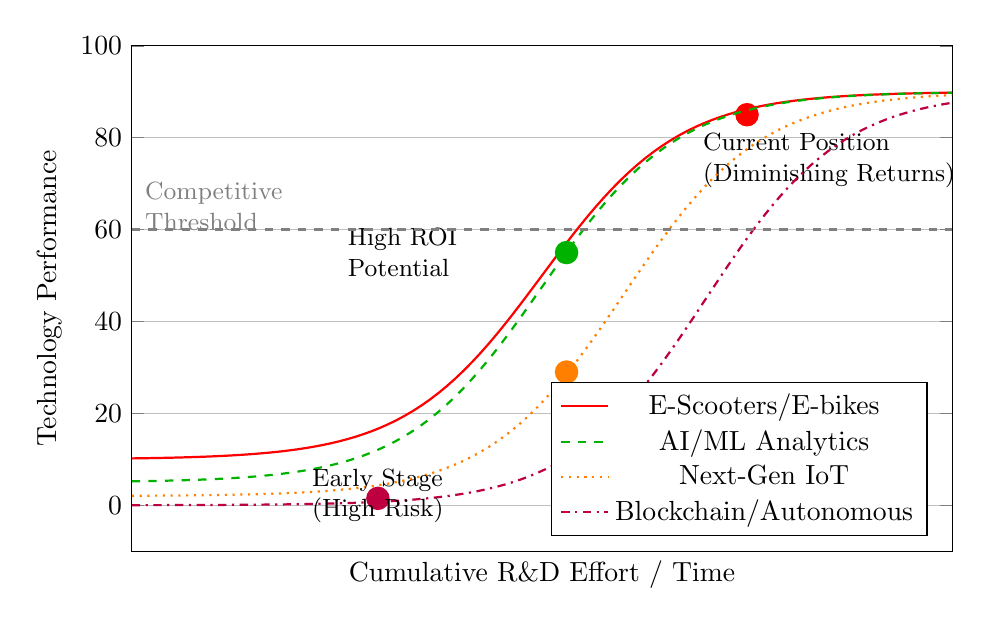
\begin{tikzpicture}
\begin{axis}[
    width=12cm,
    height=8cm,
    xlabel={Cumulative R\&D Effort / Time},
    ylabel={Technology Performance},
    xmin=0, xmax=10,
    ymin=-10, ymax=100,
    xtick=\empty,
    ytick={0,20,40,60,80,100},
    grid=major,
    legend pos=south east,
    ylabel style={align=center},
    xlabel style={align=center}
]

% Main S-curve for E-scooters/E-bikes (mature)
\addplot[
    domain=0:10,
    samples=100,
    color=red,
    thick,
    name path=scurve1
] {80/(1+exp(-1.2*(x-5))) + 10};
\addlegendentry{E-Scooters/E-bikes}

% Mark current position
\node[circle, fill=red, inner sep=3pt] at (axis cs:7.5,85) {};
\node[align=left, font=\small] at (axis cs:8.5,75) {Current Position\\(Diminishing Returns)};

% S-curve for AI/ML (mid-growth)
\addplot[
    domain=0:10,
    samples=100,
    color=green!70!black,
    thick,
    dashed
] {85/(1+exp(-1.2*(x-5))) + 5};
\addlegendentry{AI/ML Analytics}

% Mark current position for AI/ML
\node[circle, fill=green!70!black, inner sep=3pt] at (axis cs:5.3,55) {};
\node[align=left, font=\small] at (axis cs:3.3,55) {High ROI\\Potential};

% S-curve for Next-gen IoT (early growth)
\addplot[
    domain=0:10,
    samples=100,
    color=orange,
    thick,
    dotted
] {88/(1+exp(-1.2*(x-6))) + 2};
\addlegendentry{Next-Gen IoT}

% Mark current position for Next-gen IoT
\node[circle, fill=orange, inner sep=3pt] at (axis cs:5.3,29) {};

% Emerging tech curve (just starting)
\addplot[
    domain=0:10,
    samples=100,
    color=purple,
    thick,
    dashdotted
] {90/(1+exp(-1.2*(x-7))) + 0};
\addlegendentry{Blockchain/Autonomous}

% Mark current position for emerging
\node[circle, fill=purple, inner sep=3pt] at (axis cs:3,1.5) {};
\node[align=left, font=\small] at (axis cs:3,2) {Early Stage\\(High Risk)};

% Performance threshold line
\draw[dashed, gray, thick] (axis cs:0,60) -- (axis cs:10,60);
\node[align=left, font=\small, gray] at (axis cs:1,65) {Competitive\\Threshold};

\end{axis}
\end{tikzpicture}
\end{center}
\begin{center}
\textbf{Figure 2: S-curve Positioning of Key Technologies for UrbanMove}
\end{center}




\newpage
\subsubsection{Focus strategy for the next 3 to 5 years}
Whether UrbanMove should focus on incremental improvements or radical innovation over the next 3–5 years depends on balancing short-term survival with long-term competitiveness.
\\
\textbf{Recommended Strategy}: Dual-Track Approach with Incremental Emphasis (70/30 split).
\paragraph{70\% to Incremental Innovations Rationale:} UrbanMove faces urgent pressure from competitors with superior AI/predictive analytics. The company must close this gap rapidly to maintain market position. With scooters/e-bikes in late growth/maturity, competitive advantage comes from operational excellence, not revolutionary hardware changes.
Incremental improvements in AI-driven operations (Stream 2) and IoT enhancements (Stream 3) offer clearer, faster returns compared to radical innovations.
As a company under financial pressure (rising costs, intense competition), betting heavily on unproven radical innovations could be fatal.

\paragraph{30\% to Selective Radical Innovations Rationale:} To avoid being outpaced long-term, UrbanMove must invest in emerging technologies with transformative potential. Blockchain, Edge AI, and autonomous systems could redefine mobility services. Early exploration through Stream 1 (emerging tech intelligence) and Stream 4 (crowdsourced innovation) allows UrbanMove to identify promising radical innovations without overcommitting resources.
What to avoid:
\begin{itemize}
    \item Blockchain experiments: Too early, unclear value proposition in this context
    \item Proprietary vehicle design: Market doesn't reward hardware innovation at this maturity stage
    \item Unrelated diversification: Stay focused on core micro-mobility and adjacent mobility services
\end{itemize}


\begin{center}
\begin{tabular}{|l|c|c|c|}
\hline
\textbf{Technology} & \textbf{Life Cycle Stage} & \textbf{S-Curve Position} & \textbf{Investment Priority} \\
\hline
E-Scooters/E-bikes & Late Growth/Maturity & Plateau & Low (Maintain) \\
\hline
Current Telematics & Maturity & Plateau & Low (Replace) \\
\hline
AI/ML Analytics & Mid-Growth & Steep Climb & \textbf{High (Urgent)} \\
\hline
Next-Gen IoT & Early-Mid Growth & Early Climb & \textbf{High (Strategic)} \\
\hline
Blockchain/Edge AI & Introduction & Bottom & Medium (Explore) \\
\hline
Autonomous Systems & Introduction & Bottom & Low (Monitor) \\
\hline
\end{tabular}
\end{center}


\begin{center}
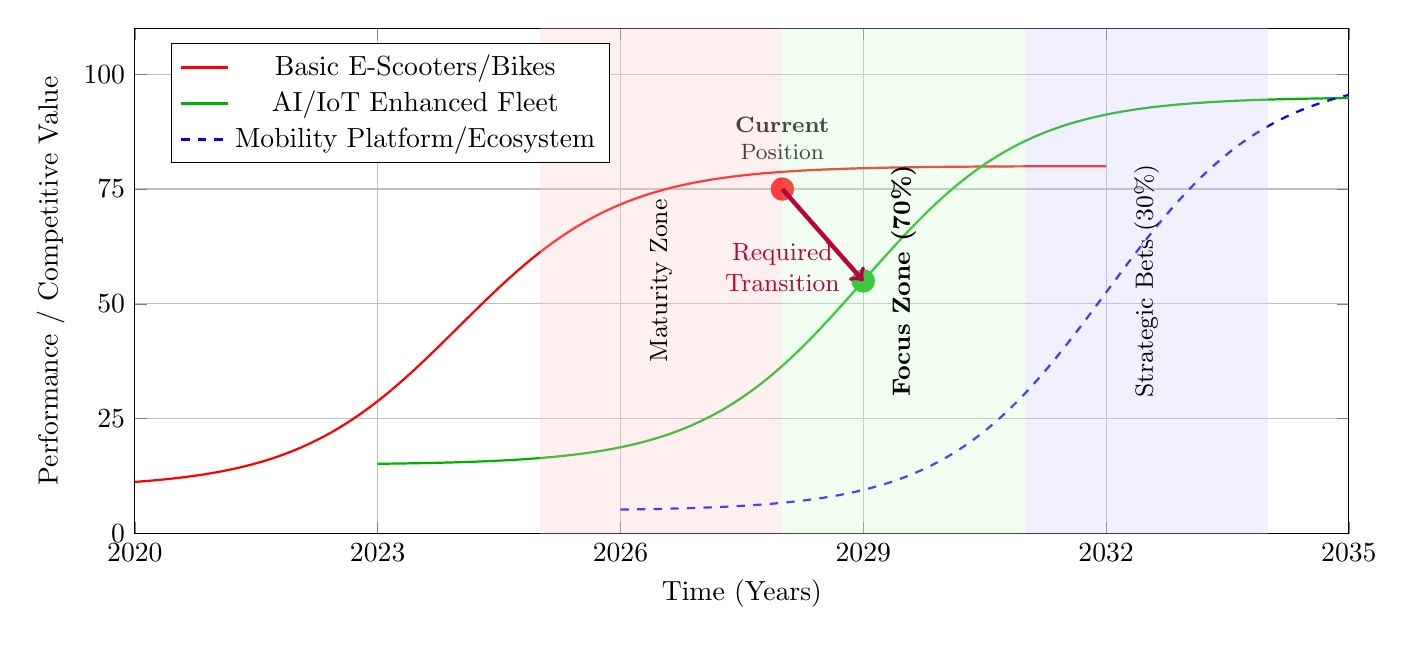
\begin{tikzpicture}
\begin{axis}[
    width=17cm,
    height=8cm,
    xlabel={Time (Years)},
    ylabel={Performance / Competitive Value},
    xmin=0, xmax=15,
    ymin=0, ymax=110,
    xtick={0,3,6,9,12,15},
    xticklabels={2020,2023,2026,2029,2032,2035},
    ytick={0,25,50,75,100},
    grid=major,
    legend pos=north west,
    ylabel style={align=center}
]

% First S-curve: Basic E-mobility (mature)
\addplot[
    domain=0:12,
    samples=100,
    color=red,
    thick
] {70/(1+exp(-1*(x-4))) + 10};
\addlegendentry{Basic E-Scooters/Bikes}

\node[circle, fill=red, inner sep=3pt] at (axis cs:8,75) {};
\node[align=center, font=\footnotesize] at (axis cs:8,86) {\textbf{Current}\\Position};

% Second S-curve: AI/IoT Enhanced (growing)
\addplot[
    domain=3:15,
    samples=100,
    color=green!70!black,
    thick
] {80/(1+exp(-1*(x-9))) + 15};
\addlegendentry{AI/IoT Enhanced Fleet}

\node[circle, fill=green!70!black, inner sep=3pt] at (axis cs:9,55) {};

% Third S-curve: Platform/Ecosystem (emerging)
\addplot[
    domain=6:15,
    samples=100,
    color=blue,
    thick,
    dashed
] {95/(1+exp(-1*(x-12))) + 5};
\addlegendentry{Mobility Platform/Ecosystem}

% Investment zones
\fill[red!20, opacity=0.3] (axis cs:5,0) rectangle (axis cs:8,110);
\node[align=center, font=\small, rotate=90] at (axis cs:6.5,55) {Maturity Zone};

\fill[green!20, opacity=0.3] (axis cs:8,0) rectangle (axis cs:11,110);
\node[align=center, font=\small, rotate=90] at (axis cs:9.5,55) {\textbf{Focus Zone (70\%)}};

\fill[blue!20, opacity=0.3] (axis cs:11,0) rectangle (axis cs:14,110);
\node[align=center, font=\small, rotate=90] at (axis cs:12.5,55) {Strategic Bets (30\%)};

% Transition arrow
\draw[->, ultra thick, purple] (axis cs:8,75) -- (axis cs:9,55);
\node[align=center, font=\small, purple] at (axis cs:8,58) {Required\\Transition};

\end{axis}
\end{tikzpicture}
\end{center}
\begin{center}
\textbf{Figure 3: Recommended Technology Transition Strategy for UrbanMove}
\end{center}

\newpage
\subsection{Selection of Innovative Projects and Proof of Concept (PoC)}


    \paragraph{Stream 1. Emerging Technology Intelligence:} Developing capabilities to identify, analyse, and adopt new disruptive technologies.
 
    \paragraph{Stream 2. AI-Driven Operations:} Implementing machine learning and predictive maintenance models to reduce fleet downtime.
 
    \paragraph{Stream 3. IoT-Enhanced Fleet Ecosystem:} Upgrading every scooter and bike with next-generation sensors, telematics, and edge-processing capabilities.

    \paragraph{Stream 4. Crowdsourced Innovation \& Funding:} Engaging users and communities in co-creating new features, and exploring crowdfunding options for green infrastructure expansion.



\subsubsection{Evaluation and Prioritization of the Project Nexus streams}
To evaluate and prioritize the four streams of Project Nexus, UrbanMove should consider the following criteria:
\\1) \textbf{Strategic Alignment:} Each stream should be evaluated based on how well it aligns with UrbanMove's strategic goals of enhancing competitiveness, improving operational efficiency, and meeting regulatory requirements.
\\2) \textbf{Risk Assessment:} Assess the technical, market, and operational risks associated with each stream. Streams with lower risk profiles may be prioritized for initial implementation.
\\3) \textbf{Resource Requirements:} Evaluate the financial, human, and technological resources required for each stream. Streams that can be executed within existing resource constraints may be prioritized.
\\4) \textbf{Time to Value:} Consider the expected time frame for each stream to deliver tangible benefits. Streams that can provide quicker returns may be prioritized to address immediate competitive pressures.
\\5) \textbf{Interdependencies:} Analyze how the streams interrelate. Some streams may enable or enhance the effectiveness of others, suggesting a logical sequence for implementation.
\\6) \textbf{Stakeholder Impact:} Evaluate the potential impact of each stream on key stakeholders, including customers, employees, and regulatory bodies. Streams that positively influence stakeholder relationships may be prioritized.



\subsubsection{Selection criteria}
Criteria for evaluating and prioritizing the streams were selected based on their relevance to UrbanMove's strategic objectives and operational context on a scale from 1 to 5 (1 = low, 5 = high)\footnote{Subjective scoring is used.}

\begin{table}[h]
\centering
\footnotesize
\begin{tabular}{|p{2.5cm}|p{1.8cm}|p{1.2cm}|p{1.8cm}|p{1.8cm}|p{1.8cm}|p{1.8cm}|p{1cm}|}
\hline
\textbf{Stream} & \textbf{Strategic Alignment} & \textbf{Risk} & \textbf{Resources} & \textbf{Time to Value} & \textbf{Inter-dependencies} & \textbf{Stakeholder} & \textbf{Total} \\
\hline
Stream 1: Emerging Tech Intelligence & & & & & & & \\
\hline
Stream 2: AI-Driven Operations & & & & & & & \\
\hline
Stream 3: IoT-Enhanced Fleet & & & & & & & \\
\hline
Stream 4: Crowdsourced Innovation & & & & & & & \\
\hline
\end{tabular}
\caption{Project Nexus Streams Evaluation Matrix}
\end{table}


\newpage
\subsubsection{PoC approach}
Outline a PoC approach for one of the streams, explaining how success should be measured.

Stream X was selected based on the evaluation matrix above.\\


\newpage
\subsection{Crowdfunding Strategies}

\subsubsection{Is crowdfunding a viable strategy?}
Critically evaluate whether crowdfunding is a viable strategy for UrbanMove’s sustainability and infrastructure initiatives.

\subsubsection{Best fit}
What type(s) of crowdfunding (donation, reward, equity, debt) would best fit their objectives?

\subsubsection{Considerations}
What risks, challenges, or ethical concerns should be considered?

\newpage
\section{Summary}

\subsection{Overall project evaluation}
\subsection{Strategic action points}


\newpage
\printbibliography
\nocite{*}

\end{document}
